\chapter{构建端盖三维模型}\label{chap:duangai}

{\bfseries 学习目标}
\begin{itemize}
\item 学习利用fillet命令绘制连接圆弧
\item 学习利用filletedge命令构建三维圆弧
\item 掌握截交线和相贯线的投影
\end{itemize}

{\bfseries 任务要求}
\begin{itemize}
\item 根据图\ref{fig:tiaoyafaduangai}所示的杯零件图,用旋转法建立调压阀杯零件的三维模型
\item 根据图\ref{fig:tiaoyafaduangai}所示的杯零件图,用实体建模法建立调压阀杯零件的三维模型
\item 根据端盖三维模型生成端盖全剖左视图。
\end{itemize}

\noindent
\begin{figure}[htbp]
\centering
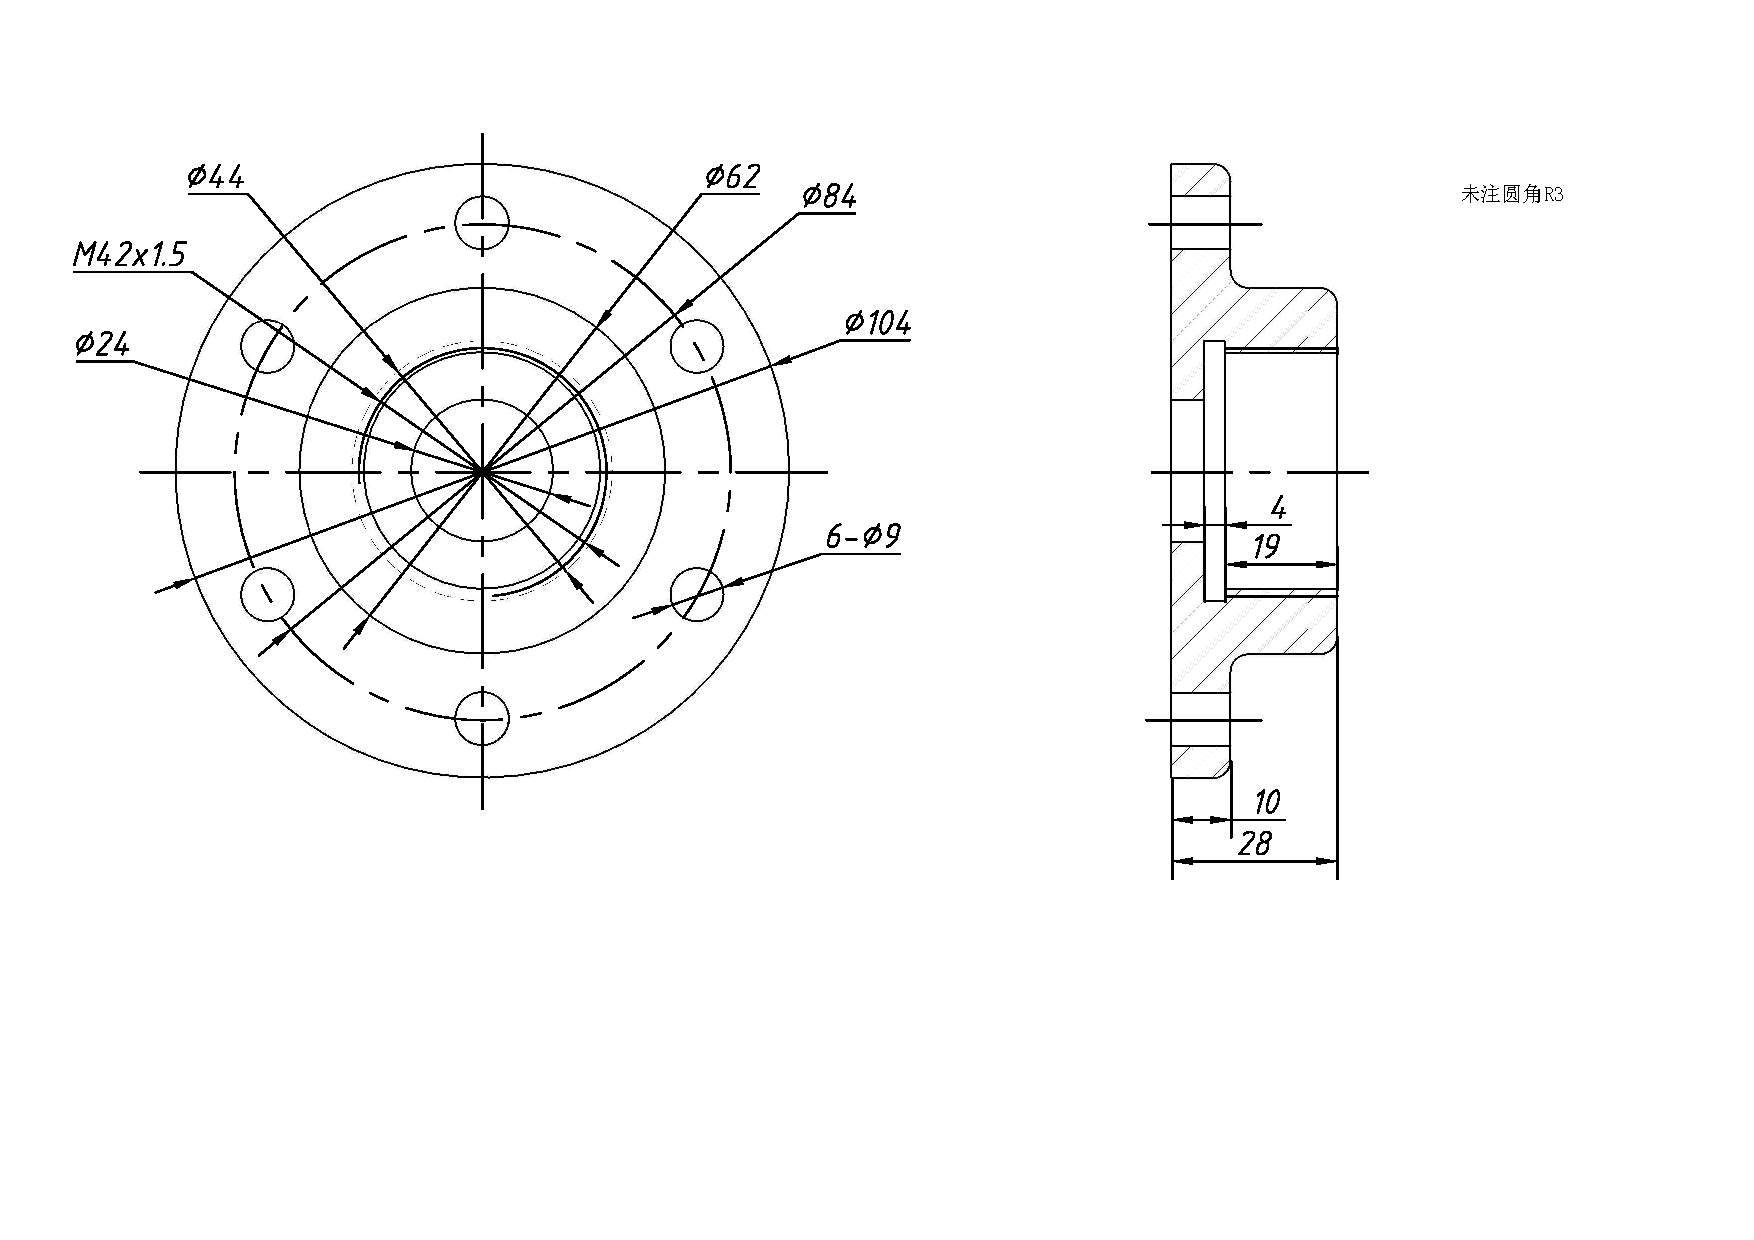
\includegraphics[scale=0.5]{tiaoyafaduangai.pdf}
\caption{端盖零件图}\label{fig:tiaoyafaduangai}
\end{figure}
\clearpage
\section{截交线与相贯线}
\section{截交体与相贯体的三视图}
\subsection{截交体}
 机器零件通常需要加工一些斜切口或开槽,这些结构可以看作是一个或多个平面切割立体而成。通常将这类立体称之为截交体。
 \subsubsection{棱柱截交体}
 图\ref{fig:jiejiao1}为正六边形棱柱截交体。该截交体的截交平面与$V$面垂直,其截交平面在俯视图和左视图中为类似形的五边形,其三视图投影如图\ref{fig:jiejiao2}所示。
 \begin{figure}[htbp]
 \centering
\subfloat[]{\label{fig:jiejiao1}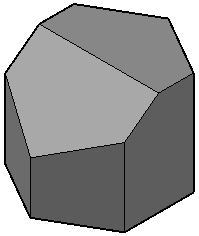
\includegraphics[scale=0.8]{jiejiao1.png}}\hspace{30pt}
\subfloat[]{\label{fig:jiejiao2}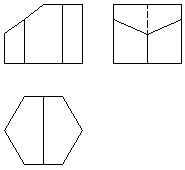
\includegraphics[scale=1]{jiejiao2.png}}
\caption{正六棱柱截交体}
\end{figure}
\subsubsection{棱锥截交体}
 图\ref{fig:jiejiao3}为正三边形棱柱截交体。该截交体的截交平面由平行于$H$面和垂直于$V$面的截交面构成,其三视图投影如图\ref{fig:jiejiao4}所示。
 \begin{figure}[htbp]
 \centering
\subfloat[]{\label{fig:jiejiao3}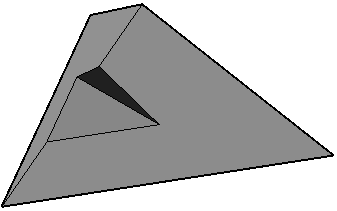
\includegraphics[scale=0.6]{jiejiao3.png}}\hspace{30pt}
\subfloat[]{\label{fig:jiejiao4}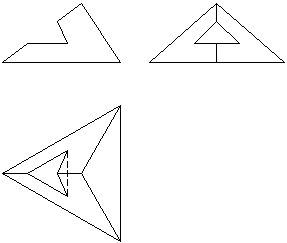
\includegraphics[scale=0.65]{jiejiao4.png}}
\caption{正六棱柱截交体}
\end{figure}
\subsubsection{圆柱截交体}
 \begin{figure}[htbp]
 \centering
\subfloat[]{\label{fig:jiejiao5}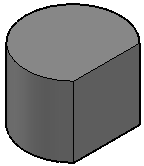
\includegraphics[scale=0.8]{jiejiao5.png}}\hspace{60pt}
\subfloat[]{\label{fig:jiejiao6}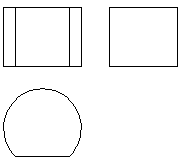
\includegraphics[scale=0.8]{jiejiao6.png}}\\
\subfloat[]{\label{fig:jiejiao7}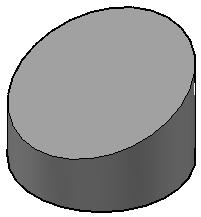
\includegraphics[scale=0.6]{jiejiao7.png}}\hspace{60pt}
\subfloat[]{\label{fig:jiejiao8}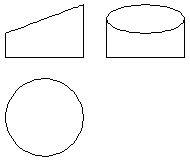
\includegraphics[scale=0.8]{jiejiao8.png}}\\
\subfloat[]{\label{fig:jiejiao9}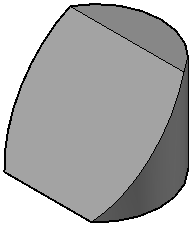
\includegraphics[scale=0.6]{jiejiao9.png}}\hspace{60pt}
\subfloat[]{\label{fig:jiejiao10}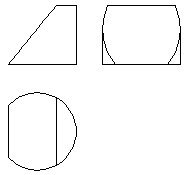
\includegraphics[scale=0.9]{jiejiao10.png}}
\caption{圆柱截交体}
\end{figure}
图\ref{fig:jiejiao5}为截交平面与轴线平,其截交线为一矩形,图\ref{fig:jiejiao6}是其三视图;图\ref{fig:jiejiao7}为截交面倾斜于轴线且不与上下表面相交,其截交线为一椭圆,图\ref{fig:jiejiao8}是其三视图;图\ref{fig:jiejiao9}为截交平面倾斜于轴线且与上下表面相交,其截交线为为复合图形,图\ref{fig:jiejiao10}是其三视图。
\clearpage
\subsubsection{圆锥截交体}
 \begin{figure}[htbp]
 \centering
\subfloat[]{\label{fig:jiejiao11}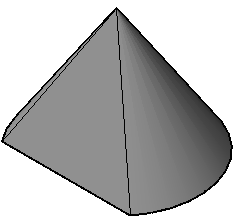
\includegraphics[scale=0.45]{jiejiao11.png}}\hspace{60pt}
\subfloat[]{\label{fig:jiejiao12}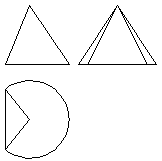
\includegraphics[scale=0.65]{jiejiao12.png}}\\
\subfloat[]{\label{fig:jiejiao13}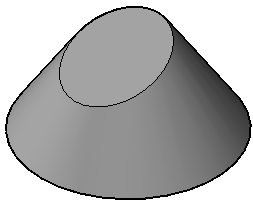
\includegraphics[scale=0.45]{jiejiao13.png}}\hspace{60pt}
\subfloat[]{\label{fig:jiejiao14}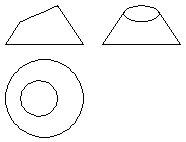
\includegraphics[scale=0.65]{jiejiao14.png}}\\
\subfloat[]{\label{fig:jiejiao15}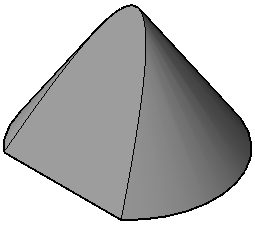
\includegraphics[scale=0.45]{jiejiao15.png}}\hspace{60pt}
\subfloat[]{\label{fig:jiejiao16}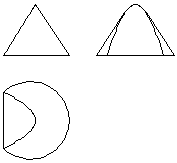
\includegraphics[scale=0.65]{jiejiao16.png}}\\
\subfloat[]{\label{fig:jiejiao17}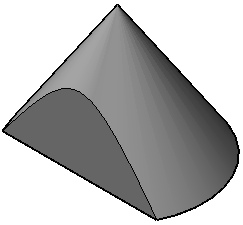
\includegraphics[scale=0.45]{jiejiao17.png}}\hspace{60pt}
\subfloat[]{\label{fig:jiejiao18}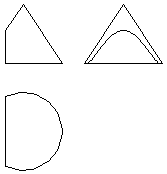
\includegraphics[scale=0.65]{jiejiao18.png}}
\caption{圆锥截交体}
\end{figure}
图\ref{fig:jiejiao11}为截交面通圆锥体锥顶,其截交线为三角形,图\ref{fig:jiejiao12}为其三视图;图\ref{fig:jiejiao13}为截面倾斜于轴线且倾斜角度大于锥角,其截交线为椭圆,图\ref{fig:jiejiao14}为其三视图;图\ref{fig:jiejiao15}为截面倾斜于轴线且倾斜角度等于锥角,其截交线为抛物线,图\ref{fig:jiejiao16}为其三视图;图\ref{fig:jiejiao17}为截面与轴线平行,其截交线为双曲线,图\ref{fig:jiejiao18}为其三视图。
\endinput
 
\subsection{相贯线}
\section{旋转建模法}
\section{旋转建模法}
\subsection{绘制左视图特征图}
\begin{procedure}
\item 设置图层。

建立“中心线”和“实线”两个图层,分别用于管理中心线和实线两类图形,并将图层设置为“中心线”层。
\item 切换视图为左视图。

\item 绘制左视图中心线。

绘制两条相互垂直的构造线型中心作为绘图参考线
\begin{lstlisting}
|命令: XLINE|
|指定点或 [水平(H)/垂直(V)/角度(A)/二等分(B)/偏移(O)]: 0,52|
|指定通过点:$ @1<0$|
|指定通过点:$ @1<90$|
|指定通过点:|
\end{lstlisting}
偏移产生$\phi 9$圆的中心线
\begin{lstlisting}
|命令: OFFSET|
|当前设置: 删除源=否  图层=源  OFFSETGAPTYPE=0|
|指定偏移距离或 [通过(T)/删除(E)/图层(L)] $<$通过$>$:42|
|选择要偏移的对象,或 [退出(E)/放弃(U)] $<$退出$>$:|
|指定要偏移的那一侧上的点,或 [退出(E)/多个(M)/放弃(U)] $<$退出$>$:|
|选择要偏移的对象,或 [退出(E)/放弃(U)] $<$退出$>$:|
\end{lstlisting}
\item 将图层切换为实线图层,绘制忽略连接圆弧的特征图,其结果如图\ref{fig:duanguaitezhengtu}所示。
\begin{figure}[htbp]
\centering
\subfloat[]{\label{fig:duanguaitezhengtu}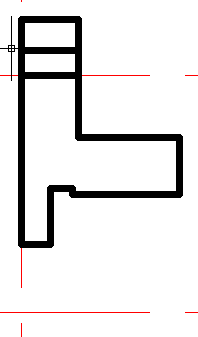
\includegraphics[scale=0.62]{duanguaitezhengtu.png}}\hspace{30pt}
\subfloat[]{\label{fig:duanguaitezhengtu1}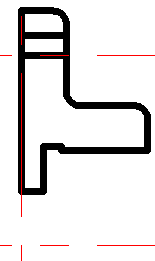
\includegraphics[scale=0.75]{duanguaitezhengtu1.png}}
\caption{端盖左视特征图绘制过程}
\end{figure}
绘主特征图。
\begin{lstlisting}
|命令: line|
|指定第一个点: 0,64|
|指定下一点或 [放弃(U)]: @0,40|
|指定下一点或 [放弃(U)]: @10,0|
|指定下一点或 [闭合(C)/放弃(U)]: @0,-21|
|指定下一点或 [闭合(C)/放弃(U)]: @18,0|
|指定下一点或 [闭合(C)/放弃(U)]: @0,-10|
|指定下一点或 [闭合(C)/放弃(U)]: @-19,0|
|指定下一点或 [闭合(C)/放弃(U)]: @0,1|
|指定下一点或 [闭合(C)/放弃(U)]: @-4,0|
|指定下一点或 [闭合(C)/放弃(U)]: @0,-10|
|指定下一点或 [闭合(C)/放弃(U)]: c|
\end{lstlisting}
绘制$\phi 9$孔特征图。
\begin{lstlisting}
|命令: rectang|
|指定第一个角点或 [倒角(C)/标高(E)/圆角(F)/厚度(T)/宽度(W)]:|
|指定另一个角点或 [面积(A)/尺寸(D)/旋转(R)]: @10,4.5|
\end{lstlisting}
\item 绘制圆弧连接,其结果如\ref{fig:duanguaitezhengtu1}所示。

绘制圆弧外连接的通常使用圆角命令。启动圆角命令的方法有:
\begin{itemize}
\item 键盘输入FILLET\index{fillet}或F。
\item 【修改】$\rightarrow$【圆角】。
\item 【修改】$\triangleright$【圆角】图标
\includegraphics[scale=0.6]{fillet.png}。
\end{itemize}
启动圆角命令后,要求选择对象。通常情况下,第一次启动圆角命令,其半径值为零。因此需要使用【半径(R)】选项先设置半径。
\begin{lstlisting}
|命令: fillet|
|当前设置: 模式 = 修剪,半径 = 0.0000|
|选择第一个对象或 [放弃(U)/多段线(P)/半径(R)/修剪(T)/多个(M)]: r| 
\end{lstlisting}
输入半圆角半径值。
\begin{lstlisting}
|指定圆角半径 $<$0.0000$>$: 3|
\end{lstlisting}
选择用于生成圆角的两边。
\begin{lstlisting}
|选择第一个对象或 [放弃(U)/多段线(P)/半径(R)/修剪(T)/多个(M)]:|
|选择第二个对象,或按住 Shift 键选择对象以应用角点或 [半径(R)]:|
\end{lstlisting}
用相同的方法生成其余两个圆角。由于圆角半径是一致的,因此不需要重复设置圆角半径,只需要直接选择用于圆角的边即可。
\begin{lstlisting}
|命令: FILLET|
|当前设置: 模式 = 修剪,半径 = 3.0000|
|选择第一个对象或 [放弃(U)/多段线(P)/半径(R)/修剪(T)/多个(M)]:|
|选择第二个对象,或按住 Shift 键选择对象以应用角点或 [半径(R)]:|
|命令: FILLET|
|当前设置: 模式 = 修剪,半径 = 3.0000|
|选择第一个对象或 [放弃(U)/多段线(P)/半径(R)/修剪(T)/多个(M)]:|
|选择第二个对象,或按住 Shift 键选择对象以应用角点或 [半径(R)]:
\end{lstlisting}
\item 面域特征图。
\begin{lstlisting}
|命令: region|
|选择对象: 指定对角点: 找到 12 个|
|选择对象:|
\end{lstlisting}
\end{procedure}
圆角命令的注意事项和技巧:
\begin{tips}
\item 如果圆角半径值为零,则不会生成圆角。
\item 圆角命令用于绘制三段圆弧内连接不是很方便,建立用使用圆或者圆弧命令,通过捕捉切点来完成。
\end{tips}

\endinput
\subsection{旋转法构建端盖三维模型}
\begin{procedure}
\item 切换西南等轴测图

\item 旋转构建端盖三维模型
旋转产生$\phi 9$圆柱体。
\begin{lstlisting}
|命令: revolve|
|当前线框密度:  ISOLINES=4,闭合轮廓创建模式 = 实体|
|选择要旋转的对象或 [模式(MO)]: MO 闭合轮廓创建模式 [实|
|体(SO)/曲面(SU)] $<$实体$>$: SO|
|选择要旋转的对象或 [模式(MO)]: 找到 1 个|
|选择要旋转的对象或 [模式(MO)]:|
|指定轴起点或根据以下选项之一定义轴 [对象(O)/X/Y/Z] $<$对象$>$:|
|指定轴端点:|
|指定旋转角度或 [起点角度(ST)/反转(R)/表达式(EX)] $<$360$>$:|
\end{lstlisting}
旋转产生端盖主特征三维模型,其结果如图\ref{fig:duangai1}所示。

\begin{lstlisting}
|命令: revolve|
|当前线框密度:  ISOLINES=4,闭合轮廓创建模式 = 实体|
|选择要旋转的对象或 [模式(MO)]: MO 闭合轮廓创建模式 [实|
|体(SO)/曲面(SU)] $<$实体$>$: SO|
|选择要旋转的对象或 [模式(MO)]: 找到 1 个|
|选择要旋转的对象或 [模式(MO)]:|
|指定轴起点或根据以下选项之一定义轴 [对象(O)/X/Y/Z] $<$对象$>$:|
|指定轴端点:near 到|
|指定旋转角度或 [起点角度(ST)/反转(R)/表达式(EX)] $<$360$>$:|
\end{lstlisting}
\item 三维阵列$\phi 9$圆柱体,其结果如图\ref{fig:duangai2}所示。
\begin{lstlisting}
|命令: 3darray|
|选择对象: 找到 1 个|
|选择对象:|
|输入阵列类型 [矩形(R)/环形(P)]$<$矩形$>$:p|
|输入阵列中的项目数目: 6|
|指定要填充的角度 (+=逆时针, -=顺时针)$ <360>$:|
|旋转阵列对象? [是(Y)/否(N)] $<Y>$:|
|指定阵列的中心点:|
|指定旋转轴上的第二点:|
\end{lstlisting}
\begin{figure}[htbp]
\centering
\subfloat[]{\label{fig:duangai1}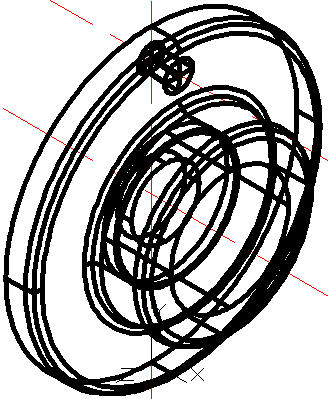
\includegraphics[scale=0.45]{duangai1.png}}\hspace{30pt}
\subfloat[]{\label{fig:duangai2}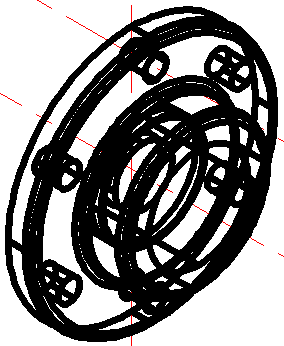
\includegraphics[scale=0.5]{duangai2.png}}\hspace{30pt}
\subfloat[]{\label{fig:duangailititu}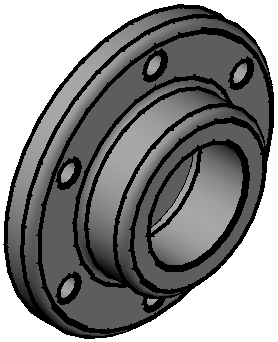
\includegraphics[scale=0.5]{duangailititu.png}}
\caption{端盖三维模型构建过程}
\end{figure}
\item 用差集操作完成三维建模操作。
\begin{lstlisting}
|命令: subtract |
|选择要从中减去的实体、曲面和面域...|
|选择对象: 找到 1 个|
|选择对象:  选择要减去的实体、曲面和面域...|
|选择对象: 找到 1 个|
|选择对象: 找到 1 个,总计 2 个|
|选择对象: 找到 1 个,总计 3 个|
|选择对象: 找到 1 个,总计 4 个|
|选择对象: 找到 1 个,总计 5 个|
|选择对象: 找到 1 个,总计 6 个|
|选择对象:|
\end{lstlisting}
\item 设置视觉样式为真实,其结果如图\ref{fig:duangailititu}所示。
\item 将端盖模型保存为“调压阀端盖立体图.dwg”。
\end{procedure}
\section{实体建模法}
\section{轴承支座立体图}

\endinput
\section{生成全剖左视图}
%%%%%%%%%%%%%%教案头%%%%%%%%%%%%%%%%%%%%%%%%%%%%%%%
\mode<article>{

\begin{longtable}{|m{20mm}|m{20mm}|m{20mm}|m{20mm}|m{20mm}|m{28mm}|}
\caption*{\huge 教案头}\\
\hline
\endfirsthead
\multicolumn{6}{l}{(续表)}\\
\hline
\endhead
\hline
\multicolumn{6}{l}{\itshape 接下一页表格.......}\\ [2ex]
\endfoot
\hline
\endlastfoot
\centering{授课单元}&\multicolumn{3}{m{60mm}|}{\centering 4.4z变换}&\centering{授课日期}&2014年06月4日 \\
\hline
\centering 授课地点 & \multicolumn{3}{m{60mm}|}{B6-204}&\centering 授课学时 & 2 \\
\hline
& \multicolumn{2}{m{40mm}|}{能力目标} & \multicolumn{2}{m{40mm}|}{知识目标}&素质目标 \\
\cline{2-6}
\centering 教学目标&\multicolumn{2}{m{40mm}|}{\begin{enumerate}
\item  能够进行离散信号的Z变换
\end{enumerate} }&\multicolumn{2}{m{40mm}|}{\begin{enumerate}
\item 了解Z变换的定义
\item 了解Z变换的求解方法
\item 了解Z变换的逆变换
\end{enumerate}} & {\qquad}\\
\hline
\centering 能力训练任务或案例 &\multicolumn{5}{m{108mm}|}{ }\\
\hline
\centering 教学重点 & \multicolumn{5}{m{108mm}|}{\begin{enumerate}
\item Z变换
\item Z变换的逆变换
\end{enumerate}}\\
\hline
\centering 教学难点与解决办法 &\multicolumn{5}{m{108mm}|}{\begin{enumerate}
\item 难点:Z变换的逆变换
\item 解决方法:实例讲解
\end{enumerate}}\\
\hline
\centering 德育内容 &\multicolumn{5}{m{108mm}|}{无}\\
\hline
 &教材 & \multicolumn{4}{m{88mm}|}{计算机控制原理与应用}\\
\cline{2-6}& 教学资源 &\multicolumn{4}{m{88mm}|}{PPT}\\
\cline{2-6}\centering 使用的教学材料& 主要教学仪器设备和工具等 &\multicolumn{4}{m{88mm}|}{投影机、MATLAB}\\
\cline{2-6}& 主要耗材 &\multicolumn{4}{m{88mm}|}{无}\\
\hline
\centering 教学模式 &\multicolumn{2}{m{40mm}|}{知识讲授}&\centering 教学手段 &\multicolumn{2}{m{48mm}|}{多媒体教学}\\
\hline
\centering 学生成果与过程考核方式 &\multicolumn{5}{m{108mm}|}{无}
\end{longtable}
\clearpage

%%%%%%%%%%%%%%%教学实施过程%%%%%%%%%%%%%%%%%%%%%%%%%%%%
\begin{landscape}

\begin{longtable}{|m{10mm}|m{50mm}|m{50mm}|m{50mm}|m{15mm}|}
\caption*{\huge 教学组织与实施}\\
\hline
\endfirsthead
\multicolumn{5}{l}{\small 接上页}\\
\hline
\multicolumn{1}{|c|}{步骤}&\multicolumn{1}{c|}{教学内容}&\multicolumn{1}{c|}{教师活动}&\multicolumn{1}{c|}{学生活动}&\multicolumn{1}{c|}{时间}\\
\hline
\endhead

\multicolumn{5}{r}{\small 接下页}\\
\endfoot
\hline
\endlastfoot
\multicolumn{1}{|c|}{步骤}&\multicolumn{1}{c|}{教学内容}&\multicolumn{1}{c|}{教师活动}&\multicolumn{1}{c|}{学生活动}&\multicolumn{1}{c|}{时间}\\\hline
讲解&\begin{enumerate}
\item Z变换的定义
\end{enumerate} &\begin{enumerate}
\item 讲解Z变换的定义
\end{enumerate} &\begin{enumerate}
\item 学生倾听并记录
\end{enumerate} &25\\\hline
讲解&\begin{enumerate}
\item Z变换的实例
\end{enumerate}
 &\begin{enumerate}
\item 讲解Z变换的例子
\end{enumerate} &\begin{enumerate}
\item 学生倾听并记录
\end{enumerate} &20 \\\hline
讲解&\begin{enumerate}
\item Z变换定理
\end{enumerate}
&\begin{enumerate}
\item 讲解Z变换定理
\end{enumerate} &\begin{enumerate}
\item 学生倾听并记录
\end{enumerate} &40 \\\hline

\centering 本次课总结(评价)&总结本课程内容 &进行知识总结 &学生倾听 &5 \\\hline
\centering 学生学习笔记或工单等检查情况&\multicolumn{4}{m{165mm}|}{\quad}\\\hline
\centering 课后作业&\multicolumn{4}{m{165mm}|}{2-28,2-29}\\\hline
\centering 教学体会&\multicolumn{4}{m{165mm}|}{\quad}\\
\end{longtable}

\end{landscape}
\clearpage
%%%%%%%%%%%%%%%%%%%%板书设计%%%%%%%%%%%%%%%%%%%%%%%%%%
\begin{center}
{\huge 板书设计}
\end{center}
}

 \begin{frame}{4.4Z变换} 
 \begin{block}{}
\[f^*(t)=\sum\limits_{k=0}^\infty f(kT)\delta(t-kT)\]
 \end{block}
 \begin{block}{拉氏变换得}
 \[F^*(s)=\sum\limits_{k=0}^\infty f(kT)e^{-kTs}\]
 \end{block}
 \end{frame}
 
 \begin{frame}
 \begin{block}{引入复变量Z}
\begin{eqnarray*}
z=e^{sT}\\
s=\frac{1}{T}\ln z
\end{eqnarray*}
\end{block}
\begin{block}{Z变换定义为}
\[F(z)=\sum\limits_{k=0}^\infty f(kT)z^{-k}\]
\end{block}
\end{frame}

\begin{frame}{Z变换定理}
\begin{block}{线性定理}
\[\pounds[af_1(t)+bf_2(t)]=aF_1(z)+bF_2(z)\]
\end{block}
\begin{block}{超前定理}
\[\pounds[f(t+nT)]=z^n\left[F(z)-\sum\limits_{q=0}^{n-1}f(qT)z^{-q}\right]\]
\end{block}

\end{frame}

\begin{frame}
\begin{block}{滞后定理}
\begin{equation*}
\pounds[f(t-nT)u(t-nT)]=z^{-n}F(z)
\end{equation*}
\end{block}
\begin{block}{有限和定理}
\begin{equation*}
\pounds\left[\sum\limits_{k=0}^nf(kT)\right]=\frac{F(z)}{1-z^{-1}}
\end{equation*}
\end{block}
\end{frame}

\begin{frame}
\begin{block}{阻尼定理}
\begin{eqnarray*}
\pounds[e^{at}f(t)]=F(e^{-aT}z)
\end{eqnarray*}
\end{block}
\begin{block}{复微分定理}
\begin{eqnarray*}
\pounds[tf(t)]=-Tz\frac{d}{dz}F(z)
\end{eqnarray*}
\end{block}
\end{frame}

\begin{frame}
\begin{block}{初值定理}
\begin{eqnarray*}
f(0)=\lim_{k\to 0}f(kT)=\lim_{z\to\infty}F(z)
\end{eqnarray*}
\end{block}
\begin{block}{终值定理}
\begin{eqnarray*}
f(\infty)=\lim_{k\to\infty}f(kT)=\lim_{z\to 1}(z-1)F(z)
\end{eqnarray*}
\end{block}
\end{frame}

\begin{frame}{Z逆变换}
\begin{block}{长除法}
先将$F(z)$展开为无穷幂级数,再逐项求$Z$逆变换,实际中只计算几项就够了。
\end{block}
\begin{block}{部分展开法}
若$F(z)$为有理函数,先将其展开,再逐项求$Z$逆变换。
\end{block}
\end{frame}
\begin{frame}{}
\begin{block}{留数法}
是一种公式法
\begin{eqnarray*}
f(kT)=\pounds^{-1}[F(z)]=\frac{1}{2\pi j}\oint_{\Gamma}F(z)z^{k-1}dz
\end{eqnarray*}
\end{block}
\begin{block}{由留数定理得}
\begin{eqnarray*}
f(kT)=f(k)=f_1+f_2+\cdots +f_n\\
\sum\limits_{k=1}^nRes[F(z)z^{k-1}]|_{z=p_i}
\end{eqnarray*}
\end{block}
\end{frame}
\begin{frame}
\begin{block}{当$p_i$为非重极点时}
\[Res[F(z)z^{k-1}]|_{z=p_i}=\lim_{z\to p_i}(z-p_i)F(z)z^{k-1}\]
则
\[f(kT)=\sum\limits_{i=1}^n\lim_{z\to p_i}(z-p_i)F(z)z^{k-1}\]
\end{block}
\end{frame}

\begin{frame}
\begin{block}{有m重极点时}
\begin{eqnarray*}
&&Res[F(z)z^{k-1}]=\\
&&\frac{1}{(m-1)!}\lim_{z\to p_j}\left\lbrace\frac{d^{m-1}}{dz^{m-1}}[(z-p_j)^mF(z)z^{k-1}]\right\rbrace\\
&&f(kT)=\sum\limits_{i=1}^{n-m}\lim_{z\to p_i}[(z-p_i)F(z)z^{k-1}+\\
&&\lim_{z\to p_j}\frac{1}{(m-1)!}\left\lbrace\frac{d^{m-1}}{dz^{m-1}}[(z-p_j)^mF(z)z^{k-1}]\right\rbrace
\end{eqnarray*}
\end{block}
\end{frame}
\begin{frame}
\begin{block}{计算法}
\begin{itemize}
\item Matlab法
\item 差分方程法
\end{itemize}
\end{block}
\end{frame}

\endinput